\section{Data preparation}
\label{sec:data_preparation}



% In previous sections, we have explained the structure of the data and how the data is labeled. In this section, we will explain how the data is prepared for training. The data preparation consists of two parts, data augmentation, and data splitting.

% After the data has been split and augmented, the data is stored in tensors of a fixed size. If an image is too small we apply a bilinear interpolation to resize the image. If an image is too large we crop the side. The images are resized to $300 \times 300$ pixels.

% \subsection{Data augmentation}
% \label{sec:data_augmentation}

% To ensure that the model is robust to different variations in the data, the data is augmented. We apply three different forms of augmentation to the data. The first form of augmentation is flipping the data. The RGB image, the depth image, and the relative joint coordinates are flipped horizontally. Furthermore, we apply random and non-random cropping to the visual data. We ensure that none of the joints are outside the image. We also apply random padding when the image is cropped. The final augmentation is Gaussian noise. We apply Gaussian noise to the RGB image and the depth image. In Figure \ref{fig:augmentation} we can see the different augmentations.

% \begin{figure}
%     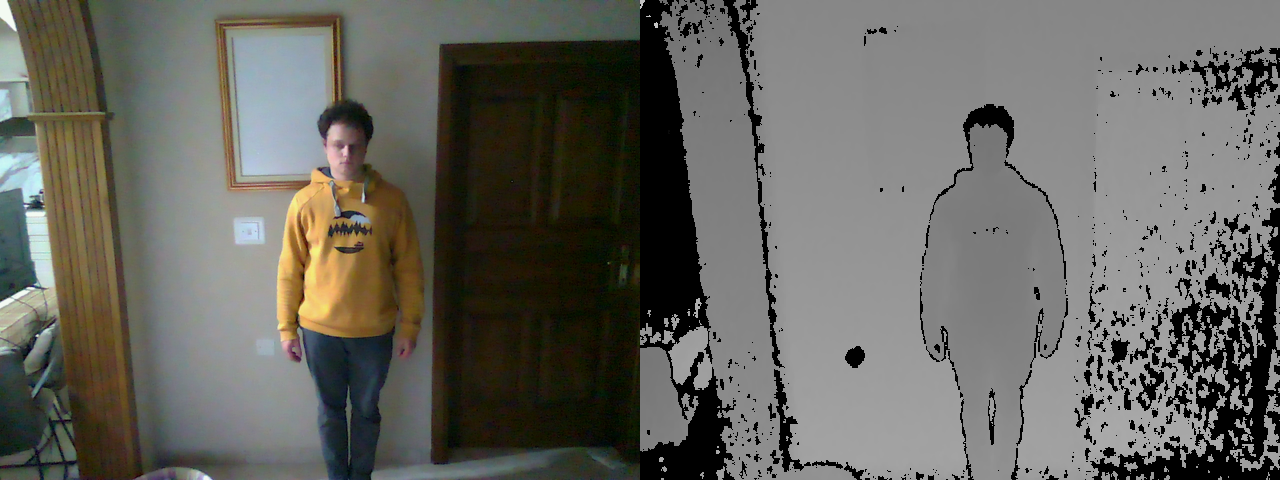
\includegraphics[width=.33\textwidth]{figures/Model/Augmentation/Original.png}\hfill
%     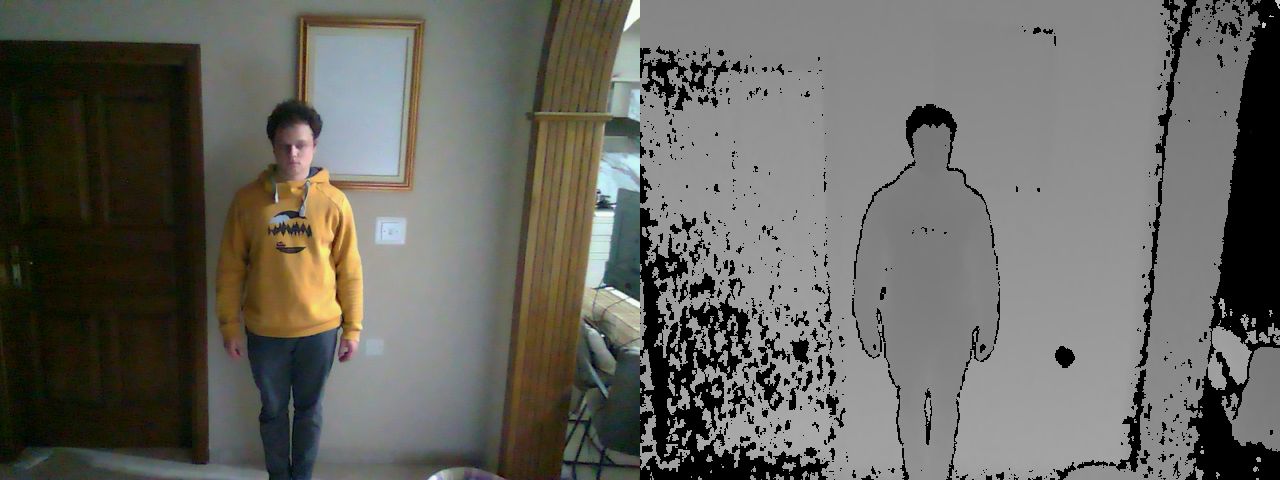
\includegraphics[width=.33\textwidth]{figures/Model/Augmentation/Flipped.png}\hfill
%     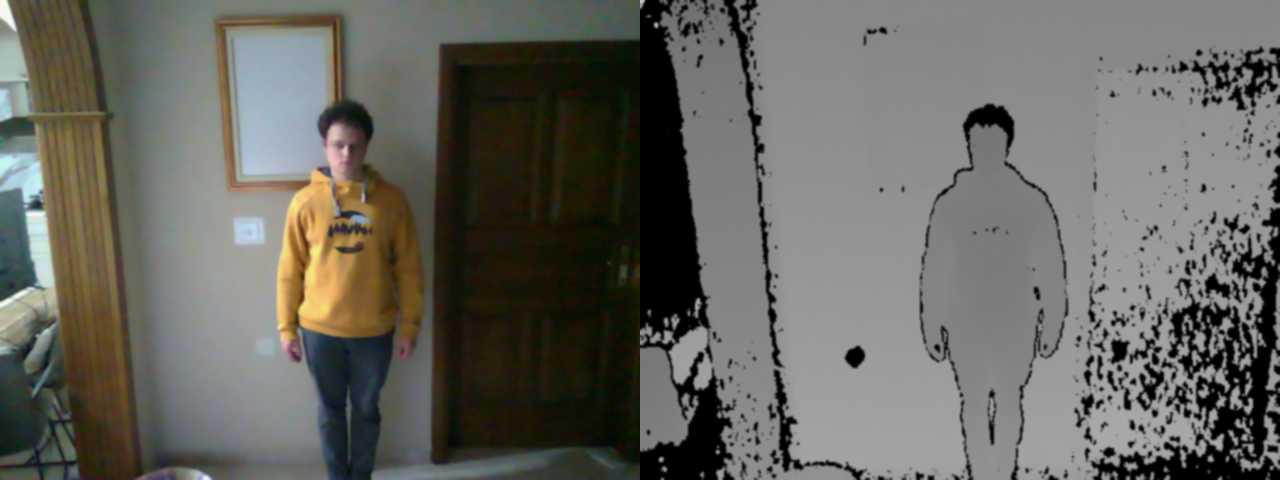
\includegraphics[width=.33\textwidth]{figures/Model/Augmentation/GaussianBlur.png}
%     \\[\smallskipamount]
%     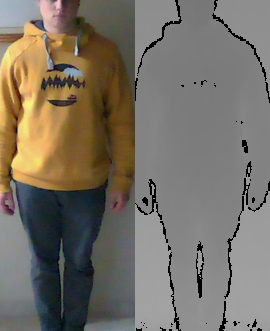
\includegraphics[width=.33\textwidth]{figures/Model/Augmentation/Cropped.png}\hfill
%     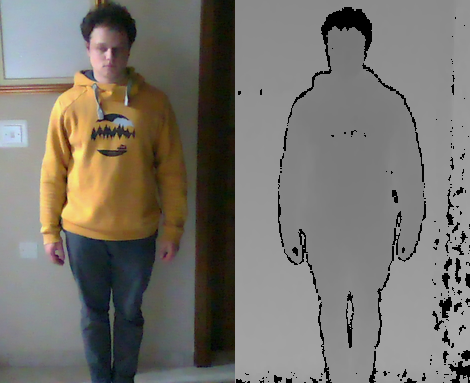
\includegraphics[width=.33\textwidth]{figures/Model/Augmentation/CroppedPad50.png}\hfill
%     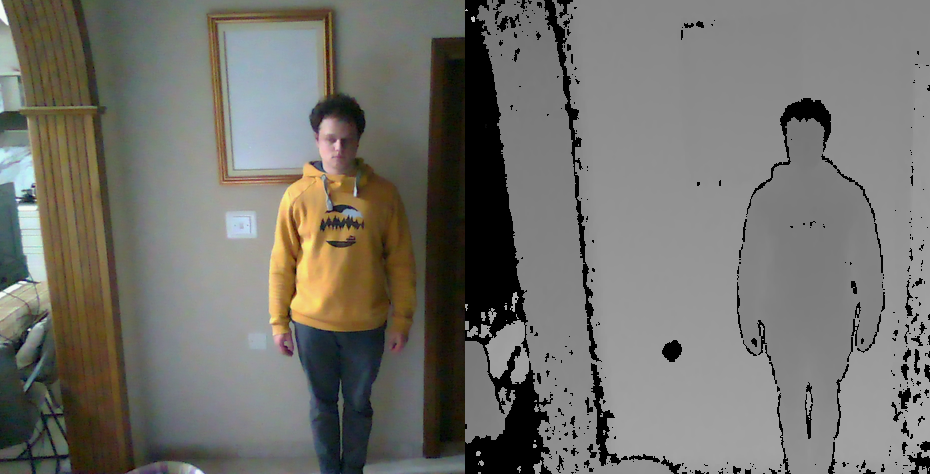
\includegraphics[width=.33\textwidth]{figures/Model/Augmentation/RandomCropped.png}
%     \caption[Data Augmentation]{Augmentation applied to a sample frame. The augmentations are; Horizontal flipping, Gaussian Blur, Exact Cropping, Exact Cropping with padding, and random Cropping respectively.}\label{fig:augmentation}
% \end{figure}


% \subsection{Data splitting}

% The data is split into two parts. The first part is the training data. The training data is used to train the model. To test the validity of the model itself, we split the data by exercise. We define 4 exercises, which are not used during training. We chose the exercises such that each exercise is in a different difficulty category, i.e. one of the exercises for testing has a trivial difficulty, one is considered as easy, and so on. With this, we try to find if our model performs better or worse with increased difficulty on unseen data.
